\documentclass[10pt,letterpaper]{article}

\usepackage{hyperref}
\usepackage{cogsci}
\usepackage{pslatex}
\usepackage{apacite}
\usepackage{graphicx}
\usepackage{caption}
\usepackage{subcaption}

\newcommand{\w}[1]{\emph{#1}}

\title{Extremely costly intensifiers are stronger than quite costly ones: a case of non-arbitrary word meanings.}
 
\author{{\large \bf Erin Bennett (erindb@stanford.edu)} \\
  Department of Psychology, 450 Serra Mall , Stanford, CA 94305
  \AND {\large \bf Noah Goodman (ngoodman@stanford.edu)} \\
  Department of Psychology, 450 Serra Mall , Stanford, CA 94305}


% 
% ## Expt. 2
% - effect of design/dependent measure?
%         - motivate new design (e.g., more adjectives)
% - design and materials
% - results and discussion
%         - as cost increases, meaning becomes more extreme
%         - (more) support for m-implicature model
%         - causal direction?
%                 - cost -> meaning?
%                 - meaning -> cost?
% 
% 
% ## General Discussion
% - m-implicature theory of intensifier interpretation
%         - benefits
%                 - single intensifier semantics
%                 - works with lassiter & goodman adjectives story
%         - model in brief?
% - further applications
%% further questions!
  
\begin{document}

\maketitle

\begin{abstract}

Abstract

\textbf{Keywords:} 
intensifiers; degree adverbs; scalar adjectives; pragmatics; m-implicature
\end{abstract}

\section{Introduction}

Introduction

% - a class of words with a similar function: intensifiers
%         - some examples
%         - differences in meaning

Intensifiers are adverbs that modify scalar adjectives to increase the degree.\footnote{The word ``intensifier'' is often used to denote the full range of degree adverbs, be they ``amplifiers'', or ``downtoners'' \cite{quirk}. The ``intensifiers'' we are looking at in this paper are, according to Quirk et al.,  ``amplifiers'' because they increase (rather than decrease) the degree to which a predicate applies. Quirk et al. also distinguish between two different kinds of amplifiers, some that increase an adjective maximally (e.g. \w{completely} and \w{utterly}) and some that merely increase (e.g. \w{greatly} and \w{terribly}). We do not make this distinction. The word ``intensifier'' is also used for a completely different linguistic phenomenon, where a reflexive is used for emphasis, e.g. ``The king himself gave the command,'' which we do not analyze in this paper.}

We first introduce a model of intensifiers which predicts an M-implicature \cite{levinson}, where more costly adjective phrases will be associated with more extreme meanings. We then confirm in two experiments that interpretations of English intensifiers in adjective phrases are indeed higher for more costly intensifiers. We conclude with a discussion of other possible explanations for this correlation and future directions.


% we could decide to have a very short section about the model.
% we take the model of the other thing which is defined by these equations.
% we assume there's a diff threshold for each sentence
% this suggests there's a route to word meanings which is not conventional lexicon thing or ideographic (form) features of words. this is a different things.
% have that as motivation. the prediction of that is that there should be an association between anything that affects costs and intensifier meaning.
% we see that correlation
% consistent wit this m-implicature story.
% it's probably too early to 
% this is a different kind of association than people have talked about.

\subsection{Motivation: possible semantics of intensifying degree adverbs}

%\subsection{Semantics of adjectives and intensifiers}
% - semantics background
%         - adjectives and thresholds
Our paper focuses on intensifying degree adverbs applied to scalar adjectives\footnote{Some of these intensifiers can also apply to verbal and nominal predicates, and different restrictions apply for different intensifiers. See \cite{bolinger} for a discussion.}. Scalar adjectives have been described as having a threshold semantics \cite{kennedy}, where for example \w{tall} means ``having a height greater than $\theta$'' and $\theta$ is a semantic variable inferred from context.
%         - lassiter & goodman: rational inference
\citeA{lassiter} give a formal model of how this threshold might be inferred, which we extend to intensifiers.

%         - intensifiers
%                 - previous proposals: restricted domain
Previous researchers have proposed that adjective phrases modified by intensifiers have the same semantics as unmodified adjectives, except with new, higher thresholds \cite{klein, kennedyMcnally, wheeler}. They suggest that the intensified thresholds are determined by first collecting the set of objects in the context class for which the bare adjective is true, and then using that as the context class to infer a new threshold, i.e. \w{very expensive laptop} means ``expensive for an expensive laptop''.
%                         - pros: domain sensitivity and increase in theta
This analysis results in the expected intensification of adjectives and is appropriately sensitive to different domains,
%                         - cons: lexical differences?
but does not in and of itself explain the difference between the strengths of, for example, \w{very expensive} and \w{phenomenally expensive}.

%                 - separate meanings?
It seems intuitively as if different intensifiers do have different strengths, and we provide further evidence of this in our experiments where participants have fairly robust judgements about the relative orderings of intensifiers. But are these differences due to learned differences in lexicon?
%                         - hard (i.e., lots) to learn
If so, it would be tasking for a learner to learn all the different lexical entries, especially since intensifiers are considered to be so numerous and so productive
% also borst: borst, eugen: die gradadverbien im englischen 1902
\cite{bolinger}.
%                         - loses within-class similarity
In addition, having different semantics for different intensifiers might be missing out the similarity among words of this class.

% - proposal in brief
%         - meaning as a function of cost
%                 - m-implicature
We hypothesize an analysis of intensifiers where each of the adjective phrases a speaker might say is associated with its own threshold, but these thresholds are systematically inferred from context and via an M-implicature (more marked intensifiers tend to correspond to higher thresholds).

%         - single intensifier semantics (increase theta)
%         - thresholds inferred
By a slight extention of \citeA{lassiter}'s model of scalar adjectives (identical to theirs except that we give different adjective phrases each their own threshold variables), we show that simply having different thresholds for different adjective phrases -- and being aware of alternative utterances and their relative communicative costs -- would be sufficient to communicate the wide range of degrees designated by intensifying degree adverbs.

The basic idea of this model is that different adjective phrases have different thresholds which must be inferred\footnote{Other versions of this model could be imagined in which the threshold for an adjective phrase is determined by the basic threshold for the adjective and some transformation on that threshold (e.g. multiplications, addition, etc.) caused by the threshold. If the transformation is mostly regular with a single parameter needing to be inferred for each intensifier, then such a model would be functionally equivalent to the one we describe here.}, but otherwise mean roughly the same thing, e.g. \w{expensive} and \w{very expensive} and \w{phenomenally expensive} all mean

\[ \lambda x . price(x) > \theta_i \]

where each intensifier (or lack thereof) gets its own threshold $\theta_i$.
Given an utterance $u_i$ (e.g. \w{an expensive laptop} or \w{a very expensive laptop}) and a set of thresholds, a literal listener $L_0$ will simply update their prior beliefs $P(d)$ about the object's degree $d$ (e.g. the laptop's price) given that the degree is greater than the threshold for that utterance.

\[ L_0(d | u_i) \propto P(d) \cdot \delta_{d > \theta_i} \]

Given a set of thresholds and alternative utterances, a speaker $S_1$ will choose utterances to have low cost $C(u)$\footnote{Though this model naturally incorporates production cost, speakers might also seek to minimize comprehension cost for their listeners as well, which would have a similar effect.}
and high probability of a literal listener correctly guessing the degree.

\[ S_1(u_i | d) \propto L_0(d | u_i) \cdot e^{-C(u_i)} \]

A pragmatic listener $L_1$ can use the prior probabilities of different degrees along with their knowledge of how much effort the speaker chose to expend to guess both what the different thresholds were for the different utterances and which degree the speaker intended to communicate.

\[ L_1(d | u_i) \propto P(d) \cdot S_1(u_i | d) \]

As an initial exploration, we simulated such a model with two intensifiers (we call them \w{very} and \w{extremely}, but we determine their costs arbitrarily) on an imaginary ``heights'' domain. The prior distribution for this domain was a multinomial peaked at 0.5 with symmetric tails. We had two different adjectives, \w{tall} and \w{short}, which determined the direction on the scale. Each combination of intensifier and adjective recieved its own threshold variable in the simulation. This simulation shows an M-implicature, with the more costly intensifiers corresponding to less probable, more extreme parts of the scale (Figure ~\ref{model}).
%``my paper is totally done'' when you expect it to be done: might actually mean that it's almost done.

% Simulation results of intensifier meanings with arbitrarily chosen ``costs'' on a discretized scale of normally distributed ``heights'' are shown in Figure~\ref{model}.

%% this simulation is actually run with the following assumptions:
% short : x < theta_short - epsilon default
% very short : x < theta_short - epsilon_very
% tall : x > theta_tall + epsilon_default
% very tall : x > theta_tall + epsilon_very
%% need to re-run with assumptions described here. will take longer, but will probably otherwise look the same.
\begin{figure}[ht]
\begin{center}
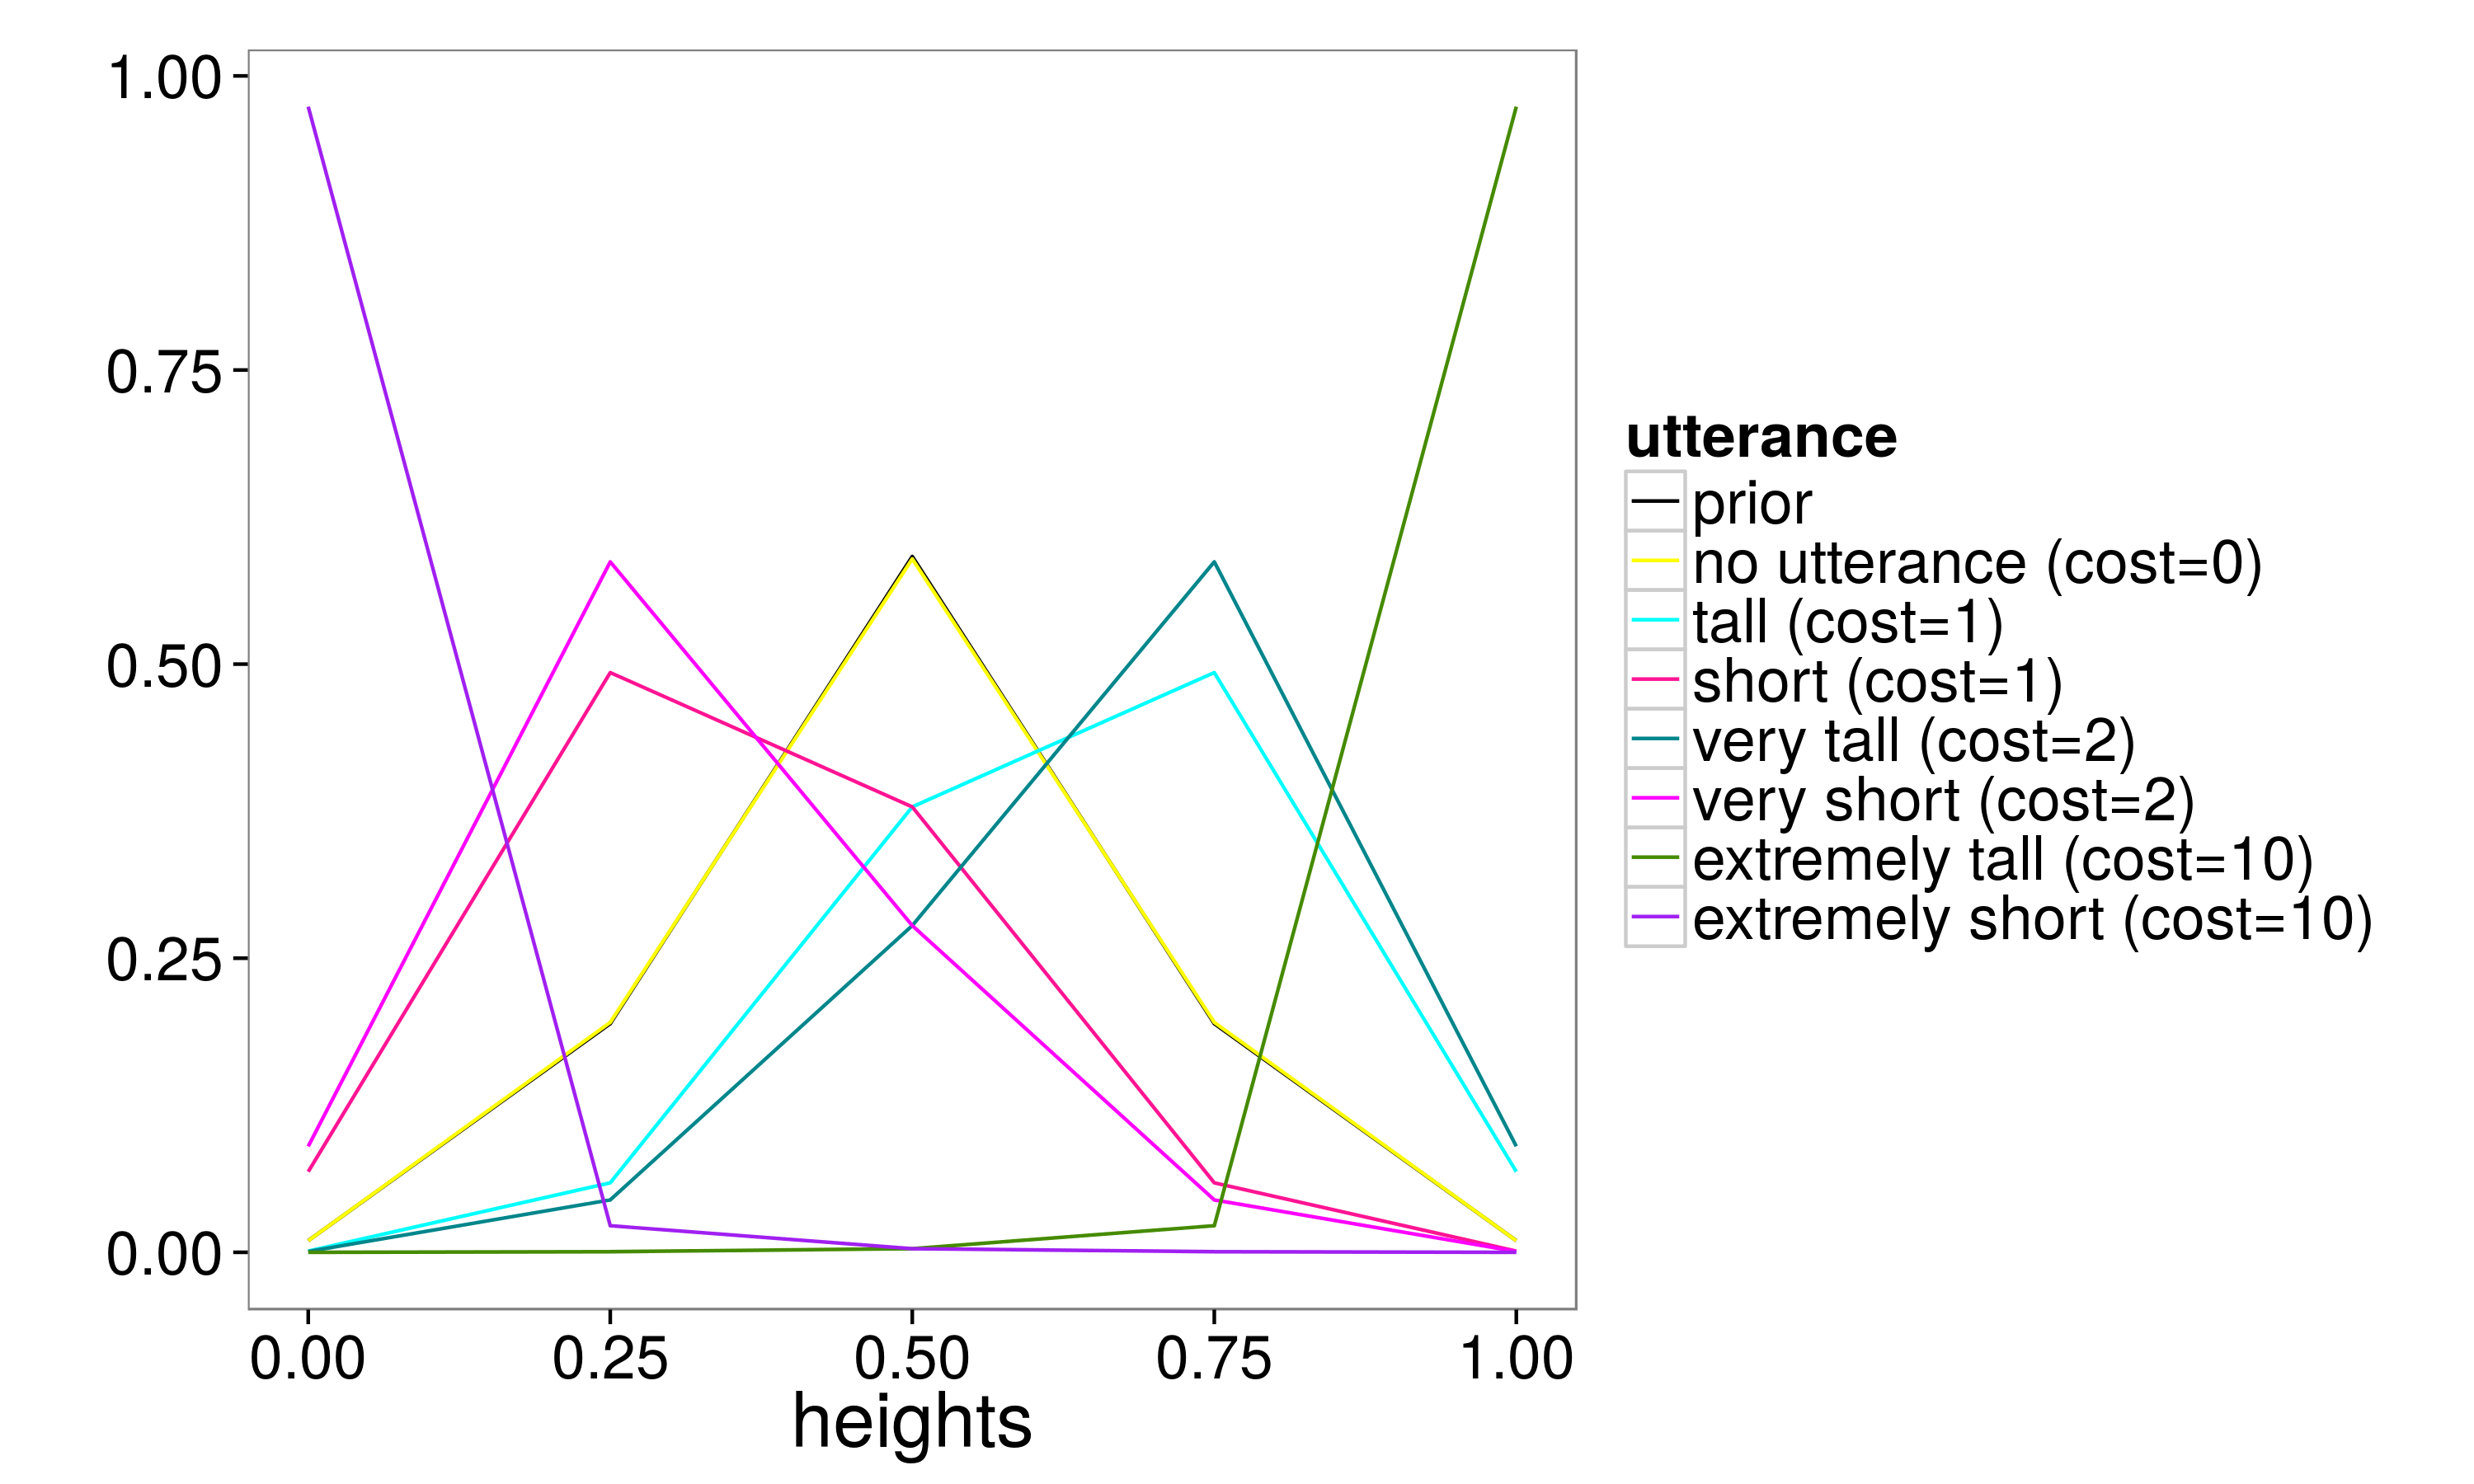
\includegraphics[width=0.48\textwidth]{analysis_files_for_writeup/images/model_results.png}
\end{center}
\caption{Modeling intensifiers as M-implicature: more costly intensifiers correspond to more extreme meanings.} 
\label{model}
\end{figure}

In Experiments 1 and 2, we test this qualitative prediction, and look at whether the cost associated with different intensifiers can predict their interpretations.

% ## Expt. 1
\section{Experiment 1}

In our first experiment, we elicited free response prices from people and determined whether these prices were correlated with independent measures of cost.

% - meaning as a function of cost?
%         - what is cost?
\subsection{Measures of cost}

Communicative cost, or markedness,
% markedness == communicative cost?
might be influenced by a variety of factors.

Peters (1994) notes that, since intensifiers often originate as qualitative adverbs and gradually shift to being primarily adverbs of degree, interlocuters might have to resolve ambiguity about which sense of the adverb is intended. Peters suggests that adverbs that are less established as intensifiers (i.e. that are still frequently used to communicate more qualitative information) will likely be more cognitively demanding to interpret as intensifiers. Given this, by our hypothesis, we would predict that such newer, ambiguous intensifiers would indicate higher degrees, all else being equal. %are there other measures worth mentioning?
%justine: ``C(u) is the psychological cost of an utterance, potentially determined by factors such as the utterance's frequency, availability, and complexity.
The extent to which a degree adverb takes a degree interpretation can be approximated by the extent to which it freely collocates with a variety of adjectives, since adverbs that are more qualitative will have more restricted collocations.

However, for the purposes of this paper, we use quantities for costs that are very easy to calculate: length (longer utterances are probably more costly)\footnote{We measure length in number of syllables, although length in characters ...} and frequency (rarer intensifiers might be less accessible and therefore harder to say or process).

%         - predictions
%                 - as cost increases, meaning becomes more extreme
We predict that as cost of an intensifier increases (i.e. as length increases and frequency decreases), its interpretation will become more extreme. This leaves open the question of their relative importance, how they combine, and what other factors (such as discuseed above) might enter into cost.

%                 - (note: not clear on causal direction (yet))
It should be noted that, as we are measuring a correlation, finding it would not confirm that an intensifier's cost actually causes its meaning. This correlation is predicted by the model sketched above, but it might be predicted by a variety of other analyses of intensifiers and their meanings. Rarity in particular might be correlated with strength of meaning merely because more extreme meanings refer to less probable things in the world, are therefore talked about less, and therefore the words with those meanings will necessarily be rarer. Although it seems reasonable to suspect that word frequencies reflect the probabilities of the real-world concepts they describe, it might also be the case that improbable things are more likely to be commented on, and so to a certain extent the frequencies of words that describe rare concepts will be inflated. Even so, this confound exists only for word frequency and not for syllable length. The length of a word seems much less likely to reflect the real-word prevalence of the concept it refers to.

% - design and materials
\subsection{Method\footnote{The full experiment can be found at \url{http://web.stanford.edu/~erindb/degree-adverbs/experiments/exp5_2014-12-01/exp5.html}}}

40 participants with US IP addresses participated in our Experiment 1 on Amazon's Mechanical Turk.

We asked participants to give us judgements of prices based on a person's description of an object that included an intensifier (Figure~\ref{exp1-q}).
There were three categories of objects (\emph{laptop}, \emph{watch}, and \emph{coffee maker}) and 40 intensifiers (see Table~\ref{exp1-intensifiers}).
We chose intensifiers that have a wide range of frequencies and excluded intensifiers that are either more commonly used to signal affect than to signal degree (e.g. ``depressingly expensive'' might indicate a degree, but it definitely indicates affect) or are ambiguous between other parts of speech (e.g. ``super'' can be used as an intensifier, as in ``super expensive'', but it can also be used as an adjective, as in ``super hero'').
Each particpant gave price judgements for every intensifier-category pairing in randomized order, for a total of 120 price judgements.
We chose the domain of price and used only the adjective ``expensive'', because price gave a quantitative scale on which to measure the different intensifers and because we thought participants would have similar enough experience with the distributions over prices for these objects.
% come to think of it, we chose those exact objects because we thought they might have bimodal priors. possibly in future experiments where the analysis would be easier if people had the same distribution as one another, we should go to something that people purchase more frequently with less ambiguity about ``what kind''... like milk, or shampoo...?

\begin{figure}[ht]
\begin{center}
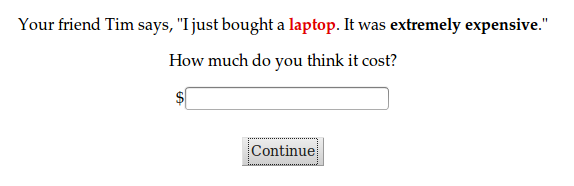
\includegraphics[width=0.4\textwidth]{analysis_files_for_writeup/images/exp1-q.png}
\end{center}
\caption{Screenshot from Experiment 1 target question.} 
\label{exp1-q}
\end{figure}

\begin{table}[ht]
 \begin{center}
 \footnotesize
  \caption{Intensifiers from Experiment 1, number of occurences in Google Web 1T 5grams corpus, and number of syllables.}
  \label{exp1-intensifiers}
  \begin{tabular}{ccc}
   \hline
   ngram & frequency & syllables \\
    \hline
    surpassingly & 11156 & 4 \\
    colossally & 11167 & 4 \\
    terrifically & 62292 & 4 \\
    frightfully & 65389 & 3 \\
    astoundingly & 73041 & 4 \\
    phenomenally & 120769 & 5 \\
    uncommonly & 135747 & 4 \\
    outrageously & 240010 & 4 \\
    fantastically & 250989 & 4 \\
    mightily & 252135 & 3 \\
    supremely & 296134 & 3 \\
    insanely & 359644 & 3 \\
    strikingly & 480417 & 3 \\
    acutely & 493931 & 3 \\
    awfully & 651519 & 3 \\
    decidedly & 817806 & 4 \\
    excessively & 877280 & 4 \\
    extraordinarily & 900456 & 6 \\
    exceedingly & 977435 & 4 \\
    intensely & 1084765 & 3 \\
    markedly & 1213704 & 3 \\
    amazingly & 1384225 & 4 \\
    radically & 1414254 & 3 \\
    unusually & 1583939 & 4 \\
    remarkably & 1902493 & 4 \\
    terribly & 1906059 & 3 \\
    exceptionally & 2054231 & 5 \\
    desperately & 2139968 & 3 \\
    utterly & 2507480 & 3 \\
    notably & 3141835 & 3 \\
    incredibly & 4416030 & 4 \\
    seriously & 12570333 & 4 \\
    truly & 19778608 & 2 \\
    significantly & 19939125 & 5 \\
    totally & 20950052 & 3 \\
    extremely & 21862963 & 3 \\
    particularly & 41066217 & 5 \\
    quite & 55269390 & 1 \\
    especially & 55397873 & 4 \\
    very & 292897993 & 2
  \end{tabular}
 \end{center}
\end{table}

\subsubsection{Corpus Methods}
%maybe have this a separate section? maybe not?

In order to measure the cost associated with different intensifiers, we collected their length in syllables and their frequencies (Table~\ref{exp1-intensifiers}).
The frequencies were collected from the Google Web 1T 5-grams database \cite{web1t5gram}\footnote{
We also ran the same analyses on frequency information collected from the Google Books American Ngrams Corpus \cite{books2011} as well, and found similar results.

In addition, we did the same using the bigram frequencies of ``\emph{[intensifer]} expensive'' rather than the unigram frequencies of the intensifiers alone. These data were much more sparse. For bigrams, we found no significant effects of surprisal using the books database and a negative effect using the web database.
}
The syllable lenths of our intensifiers and the surprisals %\todo[inline]{say what surprisal is and why we care before using it.} 
were correlated, but not strongly so (r = 0.2648144).

% - results and discussion
\subsection{Results and Discussion}

%         - as cost increases, meaning becomes more extreme
If the meaning of an intensifier is stronger for higher cost intensifiers, we would expect to find that as frequency decreases and length in syllables increases, the prices participants give will also increase. We find that this is the case.

%         - support for m-implicature model
This is the consistent with the M-implicature model introduced in this paper.


%         - effect of design/dependent measure?
%% what does this mean?

\begin{figure}[ht]
\begin{center}
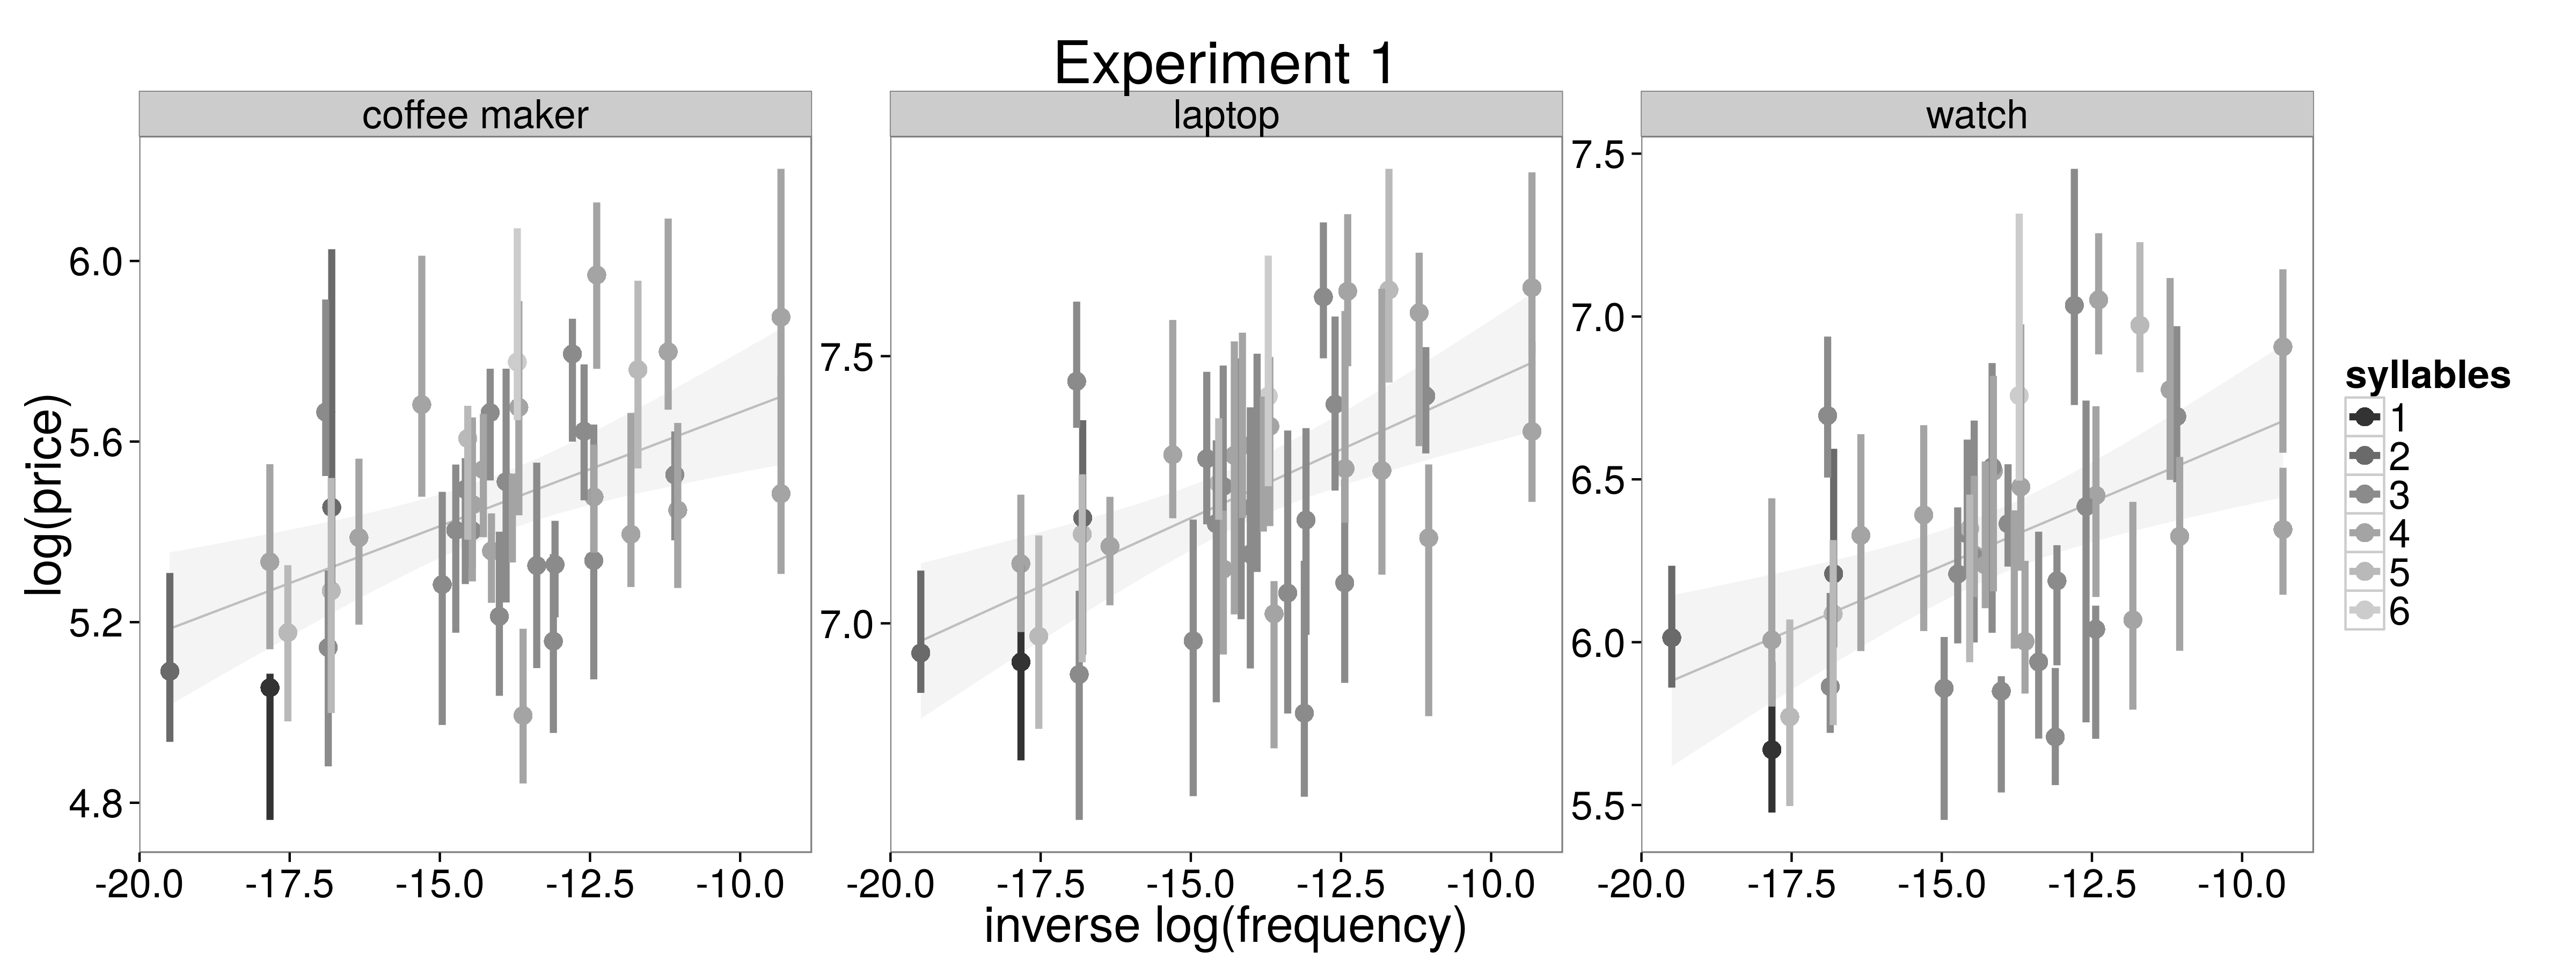
\includegraphics[width=0.48\textwidth]{analysis_files_for_writeup/images/exp1-plot.png}
\end{center}
\caption{Results of Experiment 1. As surprisal and length in syllables increase, participants' free response prices increased.} 
\label{exp1-plot}
\end{figure}

In a linear mixed effects regression with centered fixed effects of syllables and surprisal and their interaction and random intercepts and slopes for syllables and surprisal for both participant and object, we found significant main effects of surprisal (estimate=0.054, p=0.012) and syllable length  (estimate=0.093, p=0.0041) as well as a significant interaction (estimate=0.019, p=0.00018).
%anything more complicated won't converge

The interaction suggests that the function from surprisal and frequencies to cost might be multiplicative.

So intensifiers that are more surprising and longer (and therefore are more costly to utter) also tend to be interpreted as having stronger meanings.

%\todo[inline]{make a big deal}

\section{Experiment 2}

In Experiment 2, we extend our finding from Experiment 1 to other adjectival scales (in addition to ``expensive''). We use a ranking dependent measure which is more appropriate to non-quantitative scales and which we expect to be more sensitive to small differences in meaning.

\subsection{Method\footnote{The full experiment can be found at \url{http://web.stanford.edu/~erindb/degree-adverbs/experiments/exp4/exp4.html}}}

30 participants with US IP addresses participated in our Experiment 2 on Amazon's Mechanical Turk.

%\todo[inline]{introduce the idea of the ranking measure first.}
Because arranging all 40 intensifiers on a computer screen would be difficult for participants, we divided the 40 intensifiers from Experiment 1 into four lists of 10 intensifiers each (Table~\ref{exp2-intensifiers}).
Each list was randomly paired with one of four adjectives (``old'', ``expensive'', ``beautiful'', and ``tall'').
For each adjective-list pairing, participants were shown every combination of the 10 intensifiers and the one adjective on the left side of the screen.
They were asked to move the adjective phrases from the left to the right side of the screen, reordering the phrases from the lowest to the highest degree (Figure~\ref{exp2-q}).
Each participant did four trials of this process, seeing all four lists and all four adjectives.
The pairings between list and adjective were randomized between participants.
The division of the intensifiers into lists of 10 was constant, i.e. the same 10 intensifiers were always shown together to ease data analysis.

\begin{figure}[ht]
\begin{center}
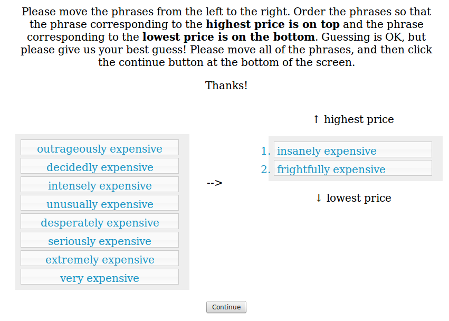
\includegraphics[width=0.4\textwidth]{analysis_files_for_writeup/images/exp2-q.png}
\end{center}
\caption{Screenshot from Experiment 2 target question.} 
\label{exp2-q}
\end{figure}

\begin{table}[ht]
\begin{center} 
\footnotesize
\caption{Intensifier Lists from Experiment 2: Rankings.} 
\label{exp2-intensifiers} 
\vskip 0.12in
%\scalebox{0.3}{
\begin{tabular}{cccc} 
\hline
List A    &  List B & List C & List D \\
\hline
surpassingly & colossally & terrifically & frightfully \\
astoundingly & phenomenally & uncommonly & outrageously \\
fantastically & mightily & supremely & insanely \\
strikingly & acutely & awfully & decidedly \\
excessively & extraordinarily & exceedingly & intensely \\
markedly & amazingly & radically & unusually \\
remarkably & terribly & exceptionally & desperately \\
utterly & notably & incredibly & seriously \\
truly & significantly & totally & extremely \\
particularly & quite & especially & very
\end{tabular}
%}
\end{center}
\end{table}

\subsection{Results and Discussion}

We ran a linear mixed effects regression with centered surprisal and syllable lengths and their interaction as fixed effects and random intercepts of intensifier list\footnote{The random intercept for intensifier list does something to standardize the rankings across the different intensifier lists. If the spacing between predictors were roughly the same across the different lists, then adding a constant value to the rankings for every element in a particular list would allow us to compare that list to another. Our predictors are not evenly spaced, so we are loosing some information in our regression, but a mixed effects model with random slopes as well as intercepts did not converge.} and adjective and random slopes for adjective to predict the ranking that participants gave the adjective phrase (the highest ranked adjective phrase in a trial got a ranking of 10, the lowest ranked adjective phrase got a ranking of 1). We found main effects of surprisal (estimate=0.46, p=4.8e-8) and syllable length (estimate=0.68, p=3.6e-10) and a significant interaction (estimate=0.079, p=0.025). Regressions on subsets of the data for each intensifier list were mostly similar, except that for intensifier lists C and D, which had smaller syllable ranges, the effects of syllable length and its interaction with surprisal were sometimes insignificant or in the opposite direction. Results were very similar across the four different adjectives.

\begin{figure}[ht]
\begin{center}

\includegraphics[width=0.48\textwidth]{analysis_files_for_writeup/images/exp2-plot.png}
\end{center}
\caption{Results of Experiment 2. As surprisal and length in syllables increase, participants' rankings increased.} 
\label{exp2-plot}
\end{figure}

Overall, we again found that participants assign stronger interpretations to intensifiers with lower frequencies and higher syllable lengths.

The relationship between frequency and interpretation might be causal, and the causal direction might be that the rarity of the word causes it to be costly to use and therefore to correspond to a stronger meaning, as in our hypothesis.
However, the causal direction could also be the opposite.
Perhaps the fact that an intensifier has a stronger meaning (which it may have gotten completely arbitrarily) causes it to be used only in extreme and unusual circumstances.
Since these circumstances rarely occur, the strong intensifier will rarely be said\footnote{This assumes that people talk about things about as frequently as they happen, which might not be the case... Isn't someone here working on how representative the internet is of what actually happens, and super rare things have an inflated presence on the web? Which is kind of evidence that people talk about extreme things more than they actually happen.}.
This seems possible, but it would not account for syllable length contributing to intensifier meaning above and beyond surprisal,  which was the case overall in Experiments 1 and 2. 

\section{Discussion}

%in general discussion / conclusion should address again the thing from the intro, also talk about other aspects of meaning (eg affect), issues with our results, and some future directions.

In conclusion, we found that frequency and syllable length can predict the interpretations of adverbs, and manipulating frequency in turn changes the interpretation, providing evidence that effective meaning is a combination of both arbitrary convention and non-arbitrary factors mediated by pragmatic inference.

%\todo[inline]{revisit our point and summarize briefly our results.}

%\todo[inline]{discuss other probable contributions to intensifier meaning: polarity, affect, others?}

%\todo[inline]{if room could say something about next steps. also relation to other's work on meaning.}

%\todo[inline]{close by restating our big picture point, that effective meaning is a combination of both arbitrary convention and non-arbitrary factors mediated by pragmatic inference.}

%\todo[inline]{conclusion}

\section{Acknowledgments}

\nocite{web1t5gram}
\nocite{lewis}
\nocite{saussure}

\bibliographystyle{apacite}

\setlength{\bibleftmargin}{.125in}
\setlength{\bibindent}{-\bibleftmargin}

\bibliography{intensifiers}

\end{document}
